%
% File naaclhlt2010.tex
%
% Contact: nasmith@cs.cmu.edu

\documentclass[11pt,letterpaper]{article}
\usepackage{naaclhlt2010}
\usepackage{times}
\usepackage{latexsym}
\usepackage{graphicx}
\setlength\titlebox{6.5cm}    % Expanding the titlebox

\title{Neural Networks for Predictive Ballistic Targeting}

\author{Vikram Chandrashekhar\\
  {\tt vchandr6@jhu.edu}
  \And
  Ran Liu \\
  {\tt rliu14@jhu.edu}}

\date{}

\begin{document}
\maketitle
\begin{abstract}
  This document contains the instructions for preparing a camera-ready
  manuscript for the proceedings of NAACL HLT 2010. The document itself conforms
  to its own specifications, and is therefore an example of what
  your manuscript should look like.  Authors are asked to conform to
  all the directions reported in this document.
\end{abstract}

\section{Introduction and Background}

The task of ballistic targeting is such- given some input, e.g. the target's current position and velocity, one must choose a firing solution such that at some time in the future, the shot fired will intercept the target's future location. This problem is primarily important to game designers interested in improving the artificial intelligence (AI) of the turret.

There are many non-machine learning (i.e linear, circular targeting) and many machine learning methods (i.e neural nets, self-organizing maps, etc) to currently solve this task \cite{Guegsen}. The current, "gold standard" for targeting methods are to compute trigonometric firing solutions using the velocity and position of the target. The two trigonometric firing solutions are linear and circular targeting; as the name implies, the linear targeting method assumes that the target will move at a constant velocity in a straight line. Similarly, the circular targeting method assumes the target is traveling in a circle of fixed radius.

The nature of the application of the problem is that the target can vary it's position very dramatically, especially when considering a human-controlled target. As such, it is important to use a method that is able to adapt to a changing underlying distribution of motion of the target. The limitation of the linear and circular models is that neither is able to adapt to changing types of motion since the underlying model (linear or circular motion) is fixed. Thus, we believe that an online machine learning algorithm is most suitable for the task. Since there may not necessarily be a linear relationship between the predictors and the output, and therefore, we require a method suitable for non linearly-separable data. The main advantage of an online algorithm is that it can adapt to changing underlying distributions of observed data and does not need to remain fixed in the case of the linear targeting.

We propose to use an artificial neural network to solve the targeting problem, as it is capable both of online learning and of classifying nonlinear data. The task at hand would be to implement a neural network algorithm that solves this task, and compare its performance against the baseline of existing non-machine learning targeting methods, e.g. linear, circular. The performance of these algorithms would then be measured using sets of targets with predefined movement patterns, as well human-controlled targets.

The features used by the neural network will be position and velocity at each time step, including a variable time step history, to predict the future motion of a target. The position and velocity will be converted to coordinates relative to the location of the turret. The relative position and velocity will then be fed into the neural network. After creating a list of possible locations of the target that cover the range of all possible locations within the bullet travel time, the output of the neural network will be the best firing solution from the candidates.

\subsection{Problem Definition}
We conceptualize the ballistic targeting problem as such:
Two entities, a turret and target, exist in a two-dimensional Cartesian space. The turret has fixed position, and exists as a point, whereas the target is represented as a circle with fixed radius, and is able to move at speeds up to a limit fixed by the parameters of the model. At regular time intervals, the turret fires projectiles, which are also represented as points, are generated at the location of the turret, and have fixed speed, but can be set to move in any direction. Collisions between projectile and target occur when the position of the projectile is contained within the boundaries of the target circle and result in the destruction of the projectile. The targeting problem is to find the set of directions for the projectiles such that the number of resultant collisions is maximized.
\section{Methods}

\subsection{Software Architecture}
In order to facilitate facile human control of targets as well as visualization of targeting algorithm results, we built a graphical user interface application, according to the model-view-controller software architecture pattern. The model portion of the application centers on the FieldModel class, which contains an object representation of the Cartesian space upon which turrets, targets, and projectiles exist. The Entity abstract superclass represents all entities which have the property of a position upon the Cartesian space, and the MoveableEntity abstract superclass represents all entities which have the properties of position and velocity. These positions are evaluated at discrete time intervals.
Turrets have TargetingAlgorithm objects bound to them, and at each firing invocation produce Projectile objects. The direction of these Projectile objects is determined by the TargetingAlgorithm which is bound to the Turret. Because targeting algorithms require access to the model state information in order to perform the necessary computations, we use the Observer design pattern/Java standard library interface, where the targeting algorithm is the observer, and the FieldModel is the observable. Therefore, whenever the state of the model is updated, all its observers are notified that an update has occurred, and the corresponding computations can be done for the next time-step. In our code, we include three implementations of TargetingAlgorithm: DirectTargeting, which commands that the turret should always fire at the current location of the target, LinearTargeting, which assumes that the target will always travel in straight lines with constant velocity, and returns FiringSolution objects accordingly, and NeuralNetworkTargeting, which reduces the ballistic targeting problem to a classification task, which is in turn handled by an artificial neural network learner. NeuralNetworkTargeting and its performance is the focus of this project.
We use the Java Swing graphical toolkit for the view portion of our application, along with the Observer pattern. The central class of the gui package, FieldView, is an Observer of the FieldModel. Therefore, when the model state is updated, the view is notified, and can be redrawn on the screen.
We have four types of controllers, one each for keyboard and mouse input, one that directly controls the FieldModel, and one that controls model playback, i.e. pauses and resumes playback. Additionally, if using target position data, rather than receiving input through the GUI, the playback controller controls the target position according to the file information. These controller objects process user input requests and invoke the appropriate methods upon model objects.

\subsection{Machine Learning Techniques}
% Explain the methods you will be using and why they are appropriate.
\subsubsection{Artificial Neural Networks}
Artificial Neural Networks (ANNs) are a set of models that are made up of many "layers" and "neurons". The "neurons" are represented by nodes in a given layer and the layers represent the sequential processing of input information as shown in Figure \ref{fig:NN}. The ANN is made up of an input layer, a series of hidden layers, and an output layer. In the case of a completely connected, feedforward ANN, all nodes in one layer are connected to all nodes in the subsequent layer. Since the targeting problem is such that all nodes require all the information from prior nodes, we implemented a fully connected, feedforward ANN.
\begin{figure}[h]
	\centering
	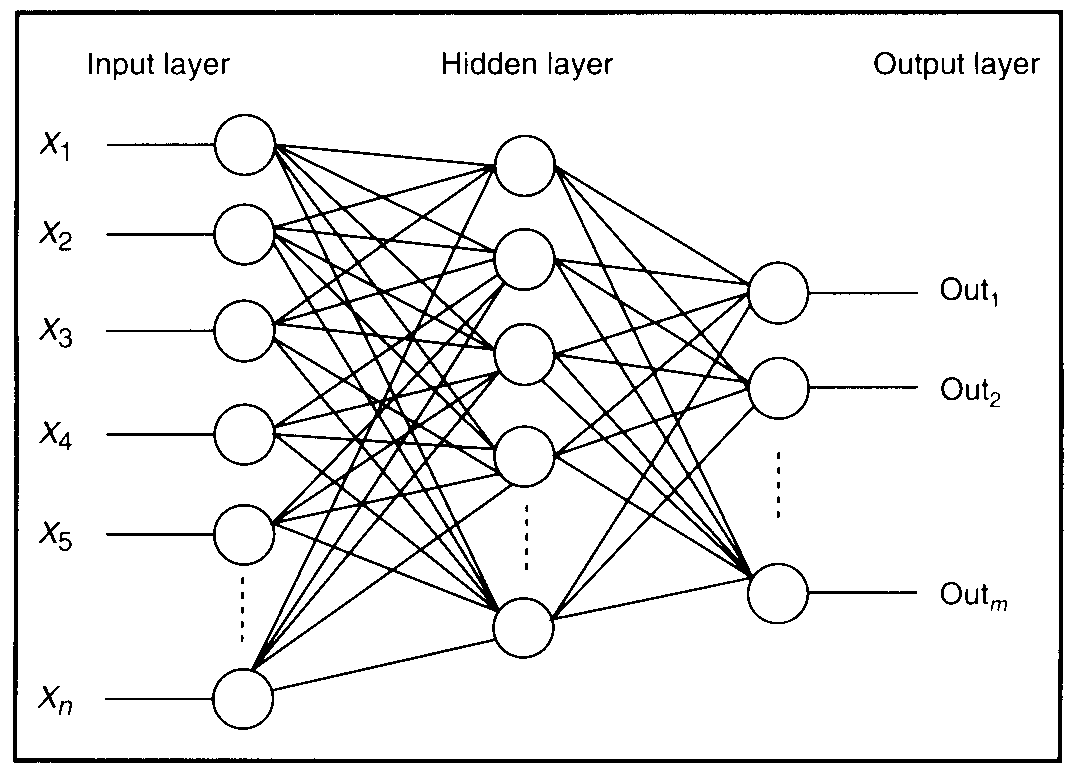
\includegraphics[scale = 0.8]{NN.png}
	\caption{Graphic representing ANN layers and nodes.}
	\label{fig:NN}
\end{figure}\\

The mathematical foundation of the ANN is  


-feature selection
-normalization
-discretizing output space

\subsection{Experimental Methods}
% What resources will you use and how will you get them?



\section{Results}


\section{Comparison to Proposal}
% What will appear in the final writeup.
\subsection{Must achieve}

We will implement multiple neural networks for predictive AI targeting for one turret and one target including all the functions that are required for training and testing. The networks will vary in depth and number of nodes and will be compared based on their accuracy.

\subsection{Expected to achieve}

We expect to create a GUI using Swing in Java that allows one to visualize the motion of the target and the bullets of the turret in real time.

\subsection{Would like to achieve}

We hope to implement a neural network for predictive targeting with multiple targets and turrets using the same neural network structure as for one target and one turret. However, we would like to explore new features outside of position and velocity at each time step. We would also like to modify our GUI in Swing to visualize this new situation.

The final writeup will include detailed derivations for the math involved in the neural networks we chose, comparisons of the accuracies of the various neural network structures explored, and the performance of our optimum choice of neural network relative to linear and circular targeting.

We will also include screenshots at various time steps of the GUI used to display the target, turret, and bullet.


\begin{thebibliography}
\bibliography{Final_Writeup}
\end{thebibliography}

\end{document}
